\documentclass[12pt]{article}
\usepackage{geometry} % see geometry.pdf on how to lay out the page. There's lots.
\geometry{a4paper} % or letter or a5paper or ... etc
% \geometry{landscape} % rotated page geometry

% See the ``Article customise'' template for come common customisations
\usepackage{color}
\usepackage{graphicx}
\usepackage{float}
\usepackage{listings}
\usepackage{caption}
\usepackage[style=british]{csquotes}
\usepackage{biblatex}
\addbibresource{coursework.bib}
\DefineBibliographyStrings{english}{bibliography = {References}}

\newcounter{nalg}[section] % defines algorithm counter for section
\renewcommand{\thenalg}{\thesection.\arabic{nalg}} %defines appearance of the algorithm counter
\DeclareCaptionLabelFormat{algocaption}{Algorithm \thenalg} % defines a new caption label as Algorithm x.y

\lstnewenvironment{algorithm}[1][]{%defines the algorithm listing environment
	\refstepcounter{nalg} %increments algorithm number
	\captionsetup{labelformat=algocaption,labelsep=colon} %defines the caption setup for: it ises label format as the declared caption label above and makes label and caption text to be separated by a ':'
	\lstset{%this is the stype
		mathescape=true,
		frame=tB,
		numbers=left, 
		numberstyle=\tiny,
		basicstyle=\scriptsize,
		breaklines=true,
		tabsize=2,
		keywordstyle=\color{black}\bfseries\em,
		keywords={IS, IF, ELSE, ENDIF, SET, FOR, ENDFOR, IN, NOT, NULL, FUNCTION, ENDFUNCTION, CLASS, ENDCLASS, MOVE, INSERT, WHILE, ENDWHILE, ROOT} %add the keywords
		numbers=left,
		xleftmargin=.02\textwidth,
		#1 % this is to add specific settings to a usage of this environment (for instance, the caption and referable label)
	}
}
{}

%%% BEGIN DOCUMENT
\begin{document}
\title{Data Structure And Algorithms - Coursework}
\author{Vishnu Sreekumar}
\date{January 2018} % delete this line to display the current date

\maketitle
\newpage
\tableofcontents
\newpage
\section{Analysis of the problem}
\paragraph The goal of the exercise is to store 10 years worth of 5 minute interval sensor readings in such a way that lookups can be done efficiently. One main characteristic of this data is that the storage requirements are constant. The client has 10 years of data and every year has 12 months. The number of days in every month is constant and so is the total number of individual sensor readings per day, which is 288. ie a reading every 5 minutes for a total 1440 minutes (60 * 24).
\paragraph{}A common requirement in the problem set is to get the sensor readings on a specific date. In some cases we also need the timestamp associated with a reading. Considering the size(1 million readings per sensor), the data needs to be organized in a way to do lookups with maximum efficiency avoiding sequential access as much possible. Another distinct requirement is to find the median Wind Speed in a given year. This requires sorting 105,120 values and we need to use an appropriate data structure to do this along with insert operation to increase efficiency. 
\paragraph{}Each input file has an year worth of data in chronological order. The date together with timestamp per line is unique within and across files. The lines are processed one by one and inserted into the proposed data structure(s). Values like maximum, average and total are calculated along with insert to avoid redundant linear parsing later. The data structure should support this using custom methods. The fact that the data set may contain duplicates has to be considered while searching and sorting. Hence the search and sort algorithms must support duplicates.

\section{Proposed Data Structures}
\paragraph{}We use a combination of Arrays, Map ADTs and Custom ADTs \cite{TEXTBOOK} to store the entire data. Let's assume that there is a wrapper function to process the input files and read one line at a time. It then separates the time stamp and sensor readings and insert them to the proposed data structures using various insertRecord() methods in the abstract data types.
\paragraph{}Wind Speed reading for a year is stored twice. One copy in a combination of a minheap and a max heap in the AnnualReadings ADT and another copy in the specific DailyReadings ADT. By splitting the wind speed readings into a maxheap and minheap of equal node count, we ensure that the middle values are always the root nodes of the respective heaps. We are sacrificing space complexity here to find the median with a constant time complexity. ie To find the median all we need to do is to get the root nodes of the heaps and find the average value.
\paragraph{}Since the keys of the input data (Year, Month, Day and Sensor Type) are pre-known and unique a {\em Map Abstract Data Type} is one of the best choices to store the data. A map lets us do the lookups with constant time complexity, ie O(1).
\paragraph{}For example to get the data for Wind Speeds on 2nd February 2014, a single lookup over a combination of map abstract data types fetches the required daily reading data structure.
\subparagraph{}
\begin{lstlisting}
READINGS[2014].monthHashmap[FEB][2][S] -> DailyReadings
\end{lstlisting}  
\paragraph{}The below diagram shows a visualization of all the data structures included.
\begin{figure}[H]
	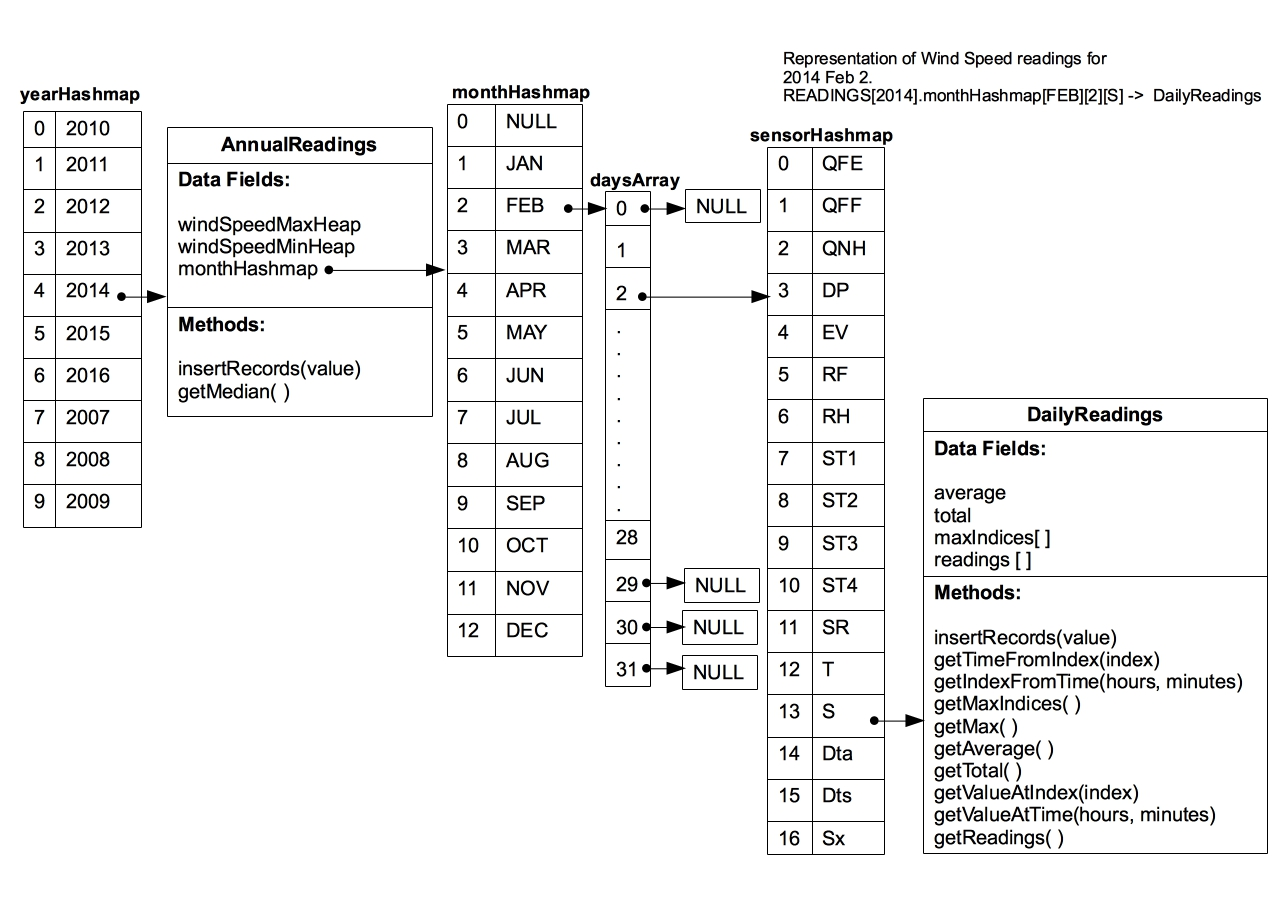
\includegraphics[width=\linewidth]{./data_structure_layout_heap.jpg}
	\caption{Wind Speeds on 2nd February 2014}
	\label{example_datastructure_layout}
\end{figure}
Individual data structures shown in Figure 1 are discussed in detail below.
\subsection{Year Map ADT}
Data for a year is stored in the {\em yearHashmap}. Since the data set is smaller (10 entries), a simple modular hashing function with a linear collision resolution can be used on an array of 10 elements.
\begin{lstlisting}
h(k) = k mod m
\end{lstlisting}
where k = year and m = 10.
\subsubsection{Lookup table}
\begin{tabular}{| c | c |}
	\hline
	Key & Index \\
	\hline
	2007 & 7 \\
	\hline
	2008  & 8 \\
	\hline
	2009 & 9 \\
	\hline
	2010 & 0 \\
	\hline
	2011 & 1 \\
	\hline
	2012 & 2 \\
	\hline
	2013 & 3 \\
	\hline
	2014 & 4 \\
	\hline
	2015 & 5 \\
	\hline
	2016 & 6 \\
	\hline
\end{tabular}
\\ \\ \\
{\em Element of yearHashmap is an object of AnnualReadings abstract data type.}
\begin{lstlisting}
yearHashmap[2014] -> AnnualReadings
\end{lstlisting}
\subsection{Annual Readings}
{\em AnnualReadings} custom ADT has the windSpeedMinHeap, windSpeedMaxHeap (used in combination to find the median) and the monthHashmap data members. It also has two methods. One to insert records to the heaps and another one to get the median wind speed. Only the Wind Speed sensor readings are inserted to the heaps in this ADT. Same readings are also stored in their corresponding DailyReadings ADT which is discussed in detail later in this section.
\paragraph{}AnnualReadings ADT has the following blueprint
\subsubsection{Data Fields}
\begin{enumerate}
	\item [--]windSpeedMinHeap
	\item [--]windSpeedMaxHeap
	\item [--]monthHashmap
\end{enumerate}
\subsubsection{Methods}
\begin{enumerate}
	\item [--]Insert new wind speed reading
	\item [--]Get median wind speed
\end{enumerate}
\subsubsection{PsuedoCode}
\begin{algorithm}[caption={Blueprint of annualReadings ADT}, label=subalgo1]
CLASS AnnualReadings():
	SET windSpeedMinHeap
	SET windSpeedMaxHeap
	SET monthHashmap

	FUNCTION insertRecord(value):
	
		// Insert value to the correct heap
		IF windSpeedMaxHeap ROOT IS NULL:
			INSERT value TO windSpeedMaxHeap
		ELSE:
			IF value > windSpeedMaxHeap ROOT:
				INSERT value to windSpeedMinHeap
			ELSE:
				INSERT value to windSpeedMaxHeap
			ENDIF
		ENDIF
		
		// Check the total number of nodes and balance the heaps if necessary
		IF COUNT(windSpeedMaxHeap) + COUNT(windSpeedMinHeap) IS EVEN:
			WHILE (COUNT(windSpeedMaxHeap) != COUNT(windSpeedMinHeap)):
				IF COUNT(windSpeedMaxHeap) > COUNT(windSpeedMinHeap):
					MOVE ROOT FROM windSpeedMaxHeap TO windSpeedMinHeap
				ELSE:
					MOVE ROOT FROM windSpeedMinHeap TO windSpeedMaxHeap
				ENDIF
			ENDWHILE
		ENDIF
	ENDFUNCTION
	
	FUNCTION getMedianWindSpeed():
		// Return the average of root nodes of min and max heaps
		RETURN ((windSpeedMinHeap ROOT) + (windSpeedMaxHeap ROOT)) / 2
	ENDFUNCTION
ENDCLASS
\end{algorithm}
\subsection{Month Map ADT}
The {\em monthHashmap} uses a custom hashing function which accepts the 3 letter string representation of month name and output the numeric value of the month. The output of this hashing function is always unique, hence there is no need for a collision resolution function. The size of the array used by this hashmap is 13 and index 0 is pointed to NULL. So that the actual values begins from 1 and goes up-to 12.
\begin{lstlisting}
h(JAN) = 1
h(FEB) = 2
h(MAR) = 3
h(APR) = 4
h(MAY) = 5
h(JUN) = 6
h(JUL) = 7
h(AUG) = 8
h(SEP) = 9
h(OCT) = 10
h(NOV) = 11
h(DEC) = 12
\end{lstlisting}
\subsubsection{Lookup Table}
\begin{tabular}{| c | c |}
	\hline
	Key & Index \\
	\hline
	JAN & 1 \\
	\hline
	FEB & 2 \\
	\hline
	MAR & 3 \\
	\hline
	APR & 4 \\
	\hline
	MAY & 5 \\
	\hline
	JUN & 6 \\
	\hline
	JUL & 7 \\
	\hline
	AUG & 8 \\
	\hline
	SEP & 9 \\
	\hline
	OCT & 10 \\
	\hline
	NOV & 11 \\
	\hline
	DEC & 12 \\
	\hline
\end{tabular}
\\ \\ \\
{\em Element of monthHashmap is a daysArray.}
\begin{lstlisting}
monthHashmap[FEB] -> daysArray[]
\end{lstlisting}

\subsection{Days Array}
The {\em daysArray} is an array of {\em sensorHashmap} values. Use of a map ADT here will be redundant and the day number can be used as the index of the array without passing it through a hashing function. The size of the array is 32, indexed (0..31), with all values initialized to NULL.
\begin{lstlisting}
daysArray = [NULL, NULL,...., NULL]
\end{lstlisting}
Initializing the array elements to NULL helps in handling the varying number of days across months. For example if the daysArray[31] is pointing to NULL, it can be safely assumed that the month has only 30 days. However while looping through the daysArray, we need to keep a separate counter variable to get the actual number of days.
\begin{algorithm}[caption={Count number of days in a given daysArray.}, label={subalgo2}]
SET counter = 0

FOR index IN 1 TO 31:
	IF daysArray[index] NOT NULL:
		SET counter = counter + 1
	ENDIF
ENDFOR	
\end{algorithm}
{\em Element of daysArray is a sensorHashmap.}
\subsection{Sensor Map ADT}
The {\em sensorHashmap} uses a custom hashing function as well. It takes the sensor type as an input and returns the index.
\begin{lstlisting}
h(QFE) = 0
h(QFF) = 1
h(QNH) = 2
h(DP) = 3
h(EV) = 4
h(RF) = 5
h(RH) = 6
h(ST1) = 7
h(ST2) = 8
h(ST3) = 9
h(ST4) = 10
h(SR) = 11
h(T) = 12
h(S) = 13
h(Dta) = 14
h(Dts) = 15
h(Sx) = 16
\end{lstlisting}
\subsubsection{Lookup Table}
\begin{tabular}{| c | c |}
	\hline
	Key & Value \\
	\hline
	QFE & 0 \\
	\hline
	QFF & 1 \\
	\hline
	QNH & 2 \\
	\hline
	DP & 3 \\
	\hline
	EV & 4 \\
	\hline
	RF & 5 \\
	\hline
	RH & 6 \\
	\hline
	ST1 & 7 \\
	\hline
	ST2 & 8 \\
	\hline
	ST3 & 9 \\
	\hline
	ST4 & 10 \\
	\hline
	SR  & 11 \\
	\hline
	T & 12 \\
	\hline
	S & 13 \\
	\hline
	Dta & 14 \\
	\hline
	Dts & 15 \\
	\hline
	Sx & 16 \\
	\hline
\end{tabular}
\\ \\ \\
{\em Element of a sensorHashmap is an object of DailyReadings ADT.}
\subsection{Daily Readings}
The goal in the design of data set for daily readings is to do the following actions efficiently:  
\begin{enumerate}
	\item Insert new item
	\item Find the max value(s) including duplicates along with the timestamp
	\item Find average value
	\item Find total
\end{enumerate}
\paragraph{}We need to use a custom Abstract Data Type with sensor readings, max, average and total as data members and a set of methods for the above calculations.
\paragraph{}Daily sensor readings are inserted to an {\em array} data field in this abstract data structure. However we need some special considerations for storing the readings.
\paragraph{}It is a requirement that we not only need the maximum values but also the timestamp associated with them. We know that readings are taken every 5 minutes and that makes a total of 288 readings per day. If we get the readings sorted by time and store them in an array of size 289 (ie index 0 - 288) starting from index 1, the nth item will be the reading at (n * 5)th minute.
\paragraph{}In 24 hr format we usually represent time as 00:00 to 23:59. That is the 288th reading in our case should actually be the first reading of the next day. The below algorithm can be tweaked to make it more realistic and support this case. However, for the sake of simplicity, we are assuming that the first reading of the day is taken at 00:05 and the last reading at 24:00. With this assumption, given an index n, we can find the corresponding time as below.\\ \\
\begin{math}
totalMinutes = n * 5 \\
hours = | totalMinutes / 60 | \\
minutes = | totalMinutes\ mod\ 60 | \\
\end{math}
\\
For example:\\
readings[15] is the reading at 75th minute or in other words, the time will be 01:15 (24 hr format). The calculation can be reversed to find the reading at a specific time as follows.\\ \\
\begin{math}
totalMinutes = (hours * 60) + minutes\\
n = totalMinutes / 5\\
value = readings[n]\\
\end{math}
\paragraph{}Average and total are calculated along with insert operation and are stored as floating point data fields. Max value(s) might have duplicates and needs to retain the timestamp information. Since we can easily find the value and time from the index of the item in the sensor readings array, the max values can be represented as an array of their indices in the sensor readings array.
\paragraph{}Putting all this together, an abstract data structure with the following blue print can be used to store the daily readings.
\subsubsection{Data fields}
\begin{enumerate}
	\item[--] Array of readings
	\item[--] Array of indices of max readings
	\item[--] Average
	\item[--] Total
\end{enumerate}
\subsubsection{Methods}
\begin{enumerate}
	\item[--] Insert new reading
	\item[--] Return array of readings
	\item[--] Return max readings array
	\item[--] Return max reading
	\item[--] Return total
	\item[--] Return average
	\item[--] Return time given an index
	\item[--] Return index given a time
\end{enumerate}
\subsubsection{Pseudo Code}
\begin{algorithm}[caption={Blueprint of dailyReadings ADT}, label=subalgo3]
CLASS DailyReadings():
	SET maxIndices = []  
	SET average = 0.0
	SET total = 0.0
	SET readings = []

	FUNCTION insertRecord(value):
		PUSH value TO readings[]
		SET lastIndex = (length of readings[]) - 1

		IF (length of maxIndices[]) > 0:
			// Get the value at current max index
			SET currentMax = readings[maxIndices[0]]
			
			IF readings[lastIndex] > currentMax:
				// Re-initialize the maxIndices array with lastIndex as the only member
				SET maxIndices = [lastIndex]
			ELSEIF readings[lastIndex] == currentMax:
				// Push lastIndex to maxIndices array if value is equal to the max value (duplicate)
				PUSH lastIndex TO maxIndices[]
			ENDIF

		ELSE:
			// If max indices array is empty add this one.
			PUSH lastIndex TO maxIndices
		ENDIF

		SET total = total + value
		SET average = total / (length of readings[])
	ENDFUNCTION

	FUNCTION getTimeFromIndex(index):
		//Assuming that time is the string representation of HH:MM in 24 hours format

		SET totalMinutes = index * 5
		SET hour = INTEGER(totalMinutes / 60)
		SET minutes = INTEGER(totalMinutes % 60)

		RETURN hour + ":" + minutes
	ENDFUNCTION

	FUNCTION getIndexFromTime(hours, minutes):
		SET totalMinutes = (hours * 60) + minutes
		SET index = totalMinutes / 5
		RETURN index
	ENDFUNCTION

	FUNCTION getMaxIndices():
		RETURN maxIndices
	ENDFUNCTION

	FUNCTION getMax():
		//Return the numeric max value (no duplicates)
		IF (length of maxIndices) > 0:
			RETURN readings[maxIndices[0]]
		ELSE:
			RETURN NULL
		ENDIF
	ENDFUNCTION

	FUNCTION getAverage():
		RETURN average
	ENDFUNCTION

	FUNCTION getTotal():
		RETURN total
	ENDFUNCTION

	FUNCTION getValueAtIndex(index):
		RETURN readings[index]
	ENDFUNCTION

	FUNCTION getValueAtTime(hours, minutes):
		SET index = getIndexFromTime(hours, minutes)
		RETURN getValueAtIndex(index)
	ENDFUNCTION

	FUNCTION getReadings():
		RETURN readings[]
	ENDFUNCTION

ENDCLASS
\end{algorithm}
\section{Algorithms}
The pseudo codes \cite{PSEUDOCODE} in this section calls the methods in the {\em DailyReadings} and {\em AnnualReadings} abstract data types. This is highlighted using in-line comments.
\subsection{The maximum wind speed of a specified month and year}
\textbf{Input}: Integer year, String month \\  
\textbf{Output}: Float windSpeed \\
\textbf{Complexity}: Constant, O(1)
\subsubsection{Pseudo Code}
\begin{algorithm}[caption={Find maximum wind speed in a given month and year}, label=algo1]
FUNCTION getMaxWindSpeed(year, month):
	SET max = 0

	FOR index IN 1 TO 31:
		SET day = READINGS[year].monthHashmap[month][index]

		IF day NOT NULL:
			SET dayMax = day[S].getMax()

			IF dayMax > max:
				SET max = dayMax
			ENDIF

		ENDIF
	ENDFOR

	RETURN max
ENDFUNCTION
\end{algorithm}
\subsection{The median wind speed of a specified year}
\textbf{Input}: Integer year \\
\textbf{Output}: Float median \\
\textbf{Complexity}: O(1)
\subsubsection{Pseudo Code}
\begin{algorithm}[caption={Find median wind speed in a given year}, label=algo2]
FUNCTION getMedian(year):
	// Call the getMedianWindSpeed method in AnnualReadings ADT
	SET median = READINGS[year].getMedianWindSpeed()
	RETURN median
ENDFUNCTION
\end{algorithm}
\subsection{Average wind speed for each month of a specified year in the order of month}
\textbf{Input}: Integer year \\
\textbf{Output}: Array of Float averageWindSpeed sorted in the oder of month\\
\textbf{Complexity}: Constant, O(1)
\subsubsection{Pseudo Code}
\begin{algorithm}[caption={Find average wind speed per month for a given year and return values in the order of month}, label=algo3]
FUNCTION getAverageWindSpeed(year):
	SET averageWindSpeed = []

	FOR month IN (JAN FEB MAR APR MAY JUN JUL AUG SEP OCT NOV DEC):
		SET monthAverageTotal = 0
		SET numberOfDays = 0

		FOR index 1 TO 31:
			SET day = READINGS[year].monthHashmap[month][index]

			IF day NOT NULL:
				SET numberOfDays = numberOfDays + 1
				// getAverage() returns the average value for the day
				SET monthAverageTotal = monthAverageTotal + day[S].getAverage()
			ENDIF
		ENDFOR

		// average of averages == average (since weight is same; 288 readings per day)
		SET monthAverage = monthAverageTotal / numberOfDays
		PUSH monthAverage TO averageWindSpeed[]
	ENDFOR

	RETURN averageWindSpeed
ENDFUNCTION
\end{algorithm}
\subsection{Total solar radiation for each month of a specified year in a descending order of the solar radiation}
\textbf{Input}: Integer year\\
\textbf{Output}: Array of Float totalSolarRadiation sorted in descending order\\
\textbf{Complexity}: Linear, O(n).
\subsubsection{Pseudo Code}
\begin{algorithm}[caption={Return total solar radion of each month in a given year; in descending order.}, label=algo4]
FUNCTION getTotalSolarRadiation(year):
	SET totalSolarRadiation = []

	FOR month IN (JAN FEB MAR APR MAY JUN JUL AUG SEP OCT NOV DEC):
		SET monthTotal = 0

		FOR index IN 1 TO 31:
			SET day = READINGS[year].monthHashmap[month][index]

			IF day NOT NULL:
				// getTotal() returns the sum of readings per day
				SET monthTotal = monthTotal + day[SR].getTotal()
			ENDIF
		ENDFOR

		// Insert monthTotal into correct position in the array
		FOR index IN 0 TO 11:
			IF totalSolarRadiation[index] IS NULL:
				SET totalSolarRadiation[index] = monthTotal
				BREAKFOR
			ELSEIF monthTotal > totalSolarRadiation[index]:
				PUSH ELEMENTS FROM INDEX UPTO END ONE STEP TO THE RIGHT
				SET totalSolarRadiation[index] = monthTotal
				BREAKFOR
			ENDIF
		ENDFOR

	ENDFOR

	RETURN totalSolarRadiation
ENDFUNCTION
\end{algorithm}
\subsection{Given a date, show the times for the highest solar radiation for that date, including duplicates, displayed in reverse chronological order}
\textbf{Input}: Integer Year, String Month, Integer Day \\
\textbf{Output}: String representation of times as HH:MM in 24 hour format in reverse chronological order\\
\textbf{Complexity}: Linear, O(n) - where n is the number of duplicates. \\
\subsubsection{Pseudo Code}
\begin{algorithm}[caption={Show the times for the highest solar radiation for a given date, including duplicates, displayed in reverse chronological order}, label=algo5]
FUNCTION getHighestSolarRadiationTimes(year, month, day):

	SET srDailyReadingsInstance = READINGS[year].monthHashmap[month][day][SR]

	// getMaxIndices() returns the array of indices of max values
	SET maxReadingsIndices = srDailyReadingsInstance.getMaxIndices()

	// getMaxIndices() method returns the array of indexes sorted in chronological order by default
	FOR index IN (length of maxReadingsIndices - 1) TO 0:
		SET maxReadingIndex = maxReadingsIndices[index]

		// getTimeFromIndex() converts the index to HH:MM string representation
		SET time = srDailyReadingsInstance.getTimeFromIndex(maxReadingIndex)
		PRINT time
	ENDFOR

ENDFUNCTION
\end{algorithm}
\section{Conclusion}
Most of the client requirements can be done in constant time complexity because of the way {\em inserts} are handled and using map abstract data type. The insert operation has a linear complexity O(n), where n is the number of readings. The operations like finding max, sum and average which themselves has a linear complexity are done along with the insert. Moreover, the readings are saved in a chronologically sorted array. This way, these operations are completely removed from the other algorithms which are called more frequently compared to insert. {\em For example, Finding the total solar radiation in a month may be called multiple times, but inserting the daily solar radiation values is only done once}. By segregating the data across various maps; lookups are also done in constant time rather than looping through the entire data one at a time.
\subsection{Space and time requirements}
\subsubsection{The maximum wind speed of a specified month and year}
Though the algorithm loops through the {\em daysArray} the relative time complexity can be considered constant because n is always between 28 and 31. Space complexity is also constant as we compare the daily maximum value with overall maximum and the same variables are re-used across the loop iterations.
\subsubsection{The median wind speed of a specified year}
To find the median we are using two different heaps in the {\em AnnualReadings} ADT. The insertRecords() member function creates these heaps by splitting the readings into two halves and storing them in a max heap and a min heap. The roots of these heaps will be mid points of all the values. So to calculate the median we need to find the average of these roots. Though the heap creation has a time complexity of O(n log n), this is handled along with insert. Hence finding the median can be done with a constant complexity O(1). Space complexity is O(2n) (or linear after removing the constant) because the values are saved twice.
\subsubsection{Average wind speed for each month of a specified year in the order of month}
The {\em monthHashmap} is visited in the order of the months and monthly averages are pushed into the output array in the same order. Hence the output array has been sorted in the required sequence. Since the {\em DailyReadings} class object has the average of readings as a data member, getting it has a constant complexity too. The space requirement is linear depending on the number of months with available readings.
\subsubsection{Total solar radiation for each month of a specified year in a descending order of the solar radiation}
Getting the total values can be done in constant complexity, however the results are sorted in place using insertion sort. Hence the algorithm has a time complexity of O(n) and space complexity of O(n).
\subsubsection{Given a date, show the times for the highest solar radiation for that date, including duplicates, displayed in reverse chronological order}
The algorithm loops through the {\em maxIndices} array, which is a data member of {\em DailyReadings} class. The iterations depends on the number of duplicate values and has a linear complexity, O(n). The {\em maxIndices} array is retrieved and stored before processing and the space complexity is also linear. \\
\printbibliography[title=References]
\end{document}